\documentclass[a4paper,11pt]{article}
\usepackage{amsmath}
\usepackage{fancyhdr}
\usepackage{graphicx}
\usepackage{url}
\usepackage{float}
\usepackage{amsmath}
\usepackage[margin=1in]{geometry}
%\usepackage[top=.6in, bottom=.8in, left=.8in, right=.8in]{geometry}

% \floatstyle{boxed}
% \restylefloat{figure}
%==== Insert cool image between title and authors ====%
\title{Using 3D Models and Computer Vision Algorithms to \\ Implement Monte Carlo Localization}
\author{ \\[7in]  John Allard, Alex Rich \\ 2014 Summer Computer Science REU, Harvey Mudd College\thanks{Funded By The NSA}}
%\date{July 6th, 2014 \\}

\begin{document}

% ==== Title Page ==== %
  \maketitle   
  %\thispagestyle{empty}
  \newpage  
  
% ==== Table Of Contents ==== %
  \tableofcontents
  \newpage

  % ==  Paper Abstract   == %
  \begin{abstract}  
  Our research group attempts to implement the Monte Carlo Localization algorithm using a 3D model of an environment and a stream of images from a robot in that environment. This entails the use of various computer vision algorithms to find and compare features between the image feed and our 3D model. The objectives of this project are to be able to localize a general actor in any 3D modeled environment quickly and accurately. This paper outlines the process that our research group has undertaken to accomplish this task and an analysis of our resulting program. 
  \end{abstract}
  
%====================================%
%===== Section 1, Introduction ===== %
%====================================%
  \section{Introduction} 
 The Monte Carlo Localization (MCL) algorithm has been used in the past\footnote{ Dieter Fox, et al. Carnegie Mellon University, University of Bonn.} to successfully localize robots using 2D maps of an environment and a stream of range sensor information. Our goal was to build off of these successes and implement a similar algorithm using a 3D map and color images from the robot as sensor data. The end goal of this project is to place a robot somewhere in an environment, request that it go somewhere, and have the robot determine where it is and how to get to the desired location.

We chose to implement the MCL algorithm using 3D models and image data because we feel that this is the way robotics is going in the future. 3D models of an environment might be hard to create now but they is constantly getting easier and cheaper create. We were lucky enough to be given a 3D imaging camera from Matterport Inc, without this device our project would not have been possible to complete. Also, cameras have become much cheaper and more portable in the last decade and there doesn't seem to be much slowing down of this, which means it will only get easier to strap a camera onto a robot for use in localization. The combination of these two trends suggests that the need for research related to localizing a robot using 3D models and image data is going to grow in the upcoming years.

 This project was undertaken by Alex Rich and John Allard during the Summer of 2014. Our research took place at Harvey Mudd College under the mentorship of Professor Zach Dodds. The funding for our project originated with the National Science Foundation. 

 The official repository for everything related to this project, included pre-localization and during-localization programs, code documentation, and various graphical programs for viewing data related to a localization attempt is hosted here : \\
\texttt{https://github.com/jhallard/3DLocalization}

\newpage

% ==   1.1 Process Overview  == %
  \section{Monte Carlo Localization Process Overview}
%  \emph{This section is for those unfamiliar with the Monte Carlo Localization algorithm.}

The overall process of having an actor\footnote{An actor is any device that has sensors and can move around an environment, e.g. a robot.} localize itself in an environment via the MCL algorithm is comprised of many steps. A general outline of these steps is listed below.
\subsection{Pre-Localization}
 These are requirements that must be satisfied for MCL to work.
  \begin{enumerate}
  \item A map of the environment needs to be imported or constructed. 
  \item Some set of quantifiable features about the map must be chosen. This enables a comparison between sensor readings from the actor and expected sensor readings from different places in the map.
  \item This step is optional.  Features from the map are computed from many different reference points and are stored for use during the localization attempt. This limits the possible particle locations compared to generating feature data at run-time, but it reduces the computational resources needed significantly and allows one to simply look up the data in a map or container. Pre-computing features also significantly reduces the complexity of the localization source code.
  \end{enumerate}
\subsection{During Localization}
  These are the steps that the Monte Carlo Localization algorithm goes through to determine the location of an actor. Each step can be implemented in many different ways.
  \begin{enumerate}
  \item An actor is placed in the environment, and some number of guesses of where it might be are randomly generated.\footnote{The uniformity of this distribution depends on the user's previous knowledge of the actor's location.} These `guesses' we will call particles, and each particle is a data structure that contains information about its own current perspective in the environment and the sensor data it would expect to read from that perspective.
  \item The program compares the current sensor readings from the actor to the expected sensor readings for each particle, and assigns a weight to each particle based on how strongly the readings correspond to one another.
  \item A distribution is created according to the grouping and weighting of particle in the program. The more heavily weighted a particle is, the higher probability it or one of its close neighbors will be sampled from our distribution.
  \item A new set of particles are sampled from this distibution, as well as a small amount are sampled from a uniform distribution across the map. After this step the total number of particles in the program is the same as in the last step.
  \item The actor is moved to a new point in the environment via some movement command from the program. Each particle has its perspective updated according to the same commands, plus some statistical error from the uncertainty in the actors movements. The expected sensor readings for each particle are also updated to correspond to its new perspective of the environment.
  \item Steps 2-4 are repeated until the actor sends an \texttt{end-program} command over a publisher or we otherwise lose contact with the actor. As long as there is a connection our program will attempt to compute the actors location and relay this data to the actor.
  \end{enumerate} 
  
The power of this algorithm comes from a few key characterstics. 
\begin{itemize}
 \item The algorithm is very general and leaves a large amount of the implementation details for the user to decide. As was stated before, this algorithm has been used in the past with both laser and sonar range data and a 2D map of an environment, in our case it was used with images from the robot and a 3D model of the environment. This algorithm is applicabile to virtually any type of sensor data, as long as this data can be compared to the expected sensor readings that various places in a map. 
 \item Secondly, from the mobility of the particles. When the actor moves, the particles move, and thus they store the probability that the actor has traveled in the path that the particle has taken. Over time, impossible paths will cause incorrect particles to be removed from the current set of guesses, leaving room for better guesses to take their place. This results in the gradual merging of particles in space to the correct location.
\end{itemize}

\newpage

%=====================================%
%===== Section 2, 3D Map Building ====%
%=====================================%
  \section{Building the 3D Map}
  We used a 3-dimensional model as our map of the actor's environment. The models tested were fully textured, high-quality laser scans of a room or series of rooms and hallways. The 3D model was important because we intended on using cameras as our sensors for the actor in our environment. The 3D map was built using a high quality camera and range scanner donated by Matterport. The camera interfaces with an iPad and scans its surroundings from multiple vantage points, eventually stitching together everything it sees into one map. %Building the 3D map would have been nearly impossible without the generosity of the Matterport team and specifically their COO Mike Beebe. They gave our research team a very well built and user-friendly 3D imaging camera which uses laser-range data to scan an enclosed space. The use of this camera saved our team countless headaches that would have incurred by attempting to stitch Kinect range-data together.
  
  \subsection{Taking the Scans}
 Our team took scans of various places on the Harvey Mudd campus, but the main environment that we wished to localize ourselves in was the 2nd floor of the Sprague building, where we work. We took 42 scans of this space, a roughly 3500 sqft floor consisting of 7-8 rooms and a large amount of non-static objects, such as chairs, robots, and whiteboards. The Matterport software allows about 100 scans for a single model, and the software bundled with the camera automatically merges these scans into one textured mesh. The software also automatically converts the data to a .obj file format for viewing on their site. We were then able to use this object file to determine features about our map.

 \begin{figure}[h!]
   \centering
     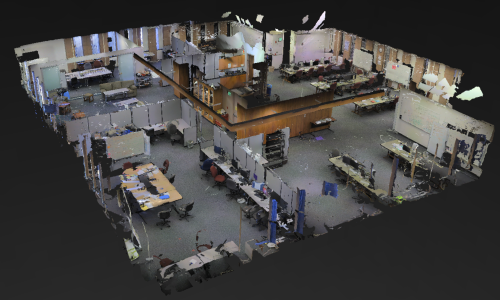
\includegraphics[height=2.3in,width=5.5in,angle=0]{../Artifacts/rp1}
 \caption{3D model of the Sprague environment.}
\end{figure}

  \subsection{Filling In the Gaps}
  Our model was inevitably left with gaps from places that were obstructed from the view of our camera. To help improve the overall quality of our map we used the Meshlab software. This allowed us to remove disconnected pieces, remove unreferenced vertices, and smoothen out some jagged areas. on top of this, we rendered the background color pink to allow us to single out features on these areas and remove them from the program. 
  
  \subsection{Creating a Database of Images from the Map}
  Our goal is to use computer vision algorithms that compare between 2D images, which meant that we had to represent our 3D map in 2D for our feature matching algorithms to work properly. To represent our 3D map as 2D information, we decided to render images from thousands of different perspectives within our map. The following steps were taken to accomplish this.
  \begin{enumerate}
  \item Establish a bounding box around our map.
  \item Define a plane that sits above and parallel to the x-y plane of our map.
  \item Define the scale of a grid imposed on this plane.
  \item Go to each grid location and render images from 8 perspectives, rotating from 0 to 360 degrees.
  \item Name the images according to their location in the map and store them for later use.
  \end{enumerate}

  This process allows us to turn our 3D model into a catalogued database of 2D images from a large amount of places within our model. From here we can use existing computer vision related algorithms (SURF, SIFT, ORB, etc.) to do the keypoint detection and feature description needed to match images with one another.


%=======================================================%
%===== Section 3, Computing Features from the Map ===== %
%=======================================================%
  \section{Computing Features from the Map}
Once we have a database of images, we must go through each image and compute a set of general feature data about each picture. This is done before localization because computing features is fairly computationally intensive, and doing so during runtime slows localization down. During the boot phase of localization, we load all features into a map.

  \subsection{Types of Features}
There are a variety of features that can be used when describing an image. In its current state, the project uses extracted SURF features as well as grayscale and black and white images.

SURF (Speeded Up Robust Features) is a feature detection algorithm that detects similar features as SIFT (Scale-Invariant Feature Transform). SURF detects interesting keypoints in an image. Using OpenCV, we can detect these points, describe them, and eventually compare two keypoints.

The Grayscale image is a highly coarse image that simply splits an image into a grid, then computes the average intensity inside each grid square. From this image, we can compute the black and white ``above below" image. This is created by finding the average intensity of the grayscale, then determining if a square is either higher or lower than this. If a square is higher, it is colored white, otherwise it is colored black.

  \subsection{Storing the Features}
The precomputed features are stored in a yaml file. OpenCV has built in storage methods, which makes this a simple process. Because each perspective has its own file for storing keypoints|in addition to its own file for grayscale and black and white images|the filename contains the meta information about each description. The program is able to load all features and know their corresponding location and orientation by first looking inside the folder to see what perspectives are available, then load into the map.

\newpage
%========================================%
%===== Section 4, MCL Implementation ====% 
%========================================%
  \section{Implementation}

 \subsection{Overview}
 This section will describe our implementation of the localization program. 
   
 \subsection{Actor Specifications}
\begin{itemize}
\item \textbf{Overview} \\
One of the main goals for our project was to be able to localize a \emph{general} actor in a \emph{general} environment. With this in mind, we tried to limit the number of requirements we impose on the movement and control of the actor. In summary, the actor must send us data from a camera and let us know its local movement coordinates, as well as listen for its global coordinates from our localization progran. All other control aspects of the actor are up to the user to decide. We have used this program successfully with both the ARDrone quad-copters and the ICreate robots, two very different robots. In our implementation, simple point to point navigation was sufficient, however a future goal is to implement the ability to make smart paths allowing the robot to go through doors and around or over tables.

\item \textbf{Communication} \\
  \begin{itemize}
  \item Publish data via two \texttt{ros::Publisher} objects. The first is for sending image data to our program, the second is to send its current movement commands to our program. 
  \item Subscribe to our data feed via a \texttt{ros::Subscriber} object. We will use this data feed to send localization data to the actor.
  \item The control code for the actor must be developed separately, the user chooses how to move the robot, we only care about localizing it in the given environment.
  \end{itemize} 
\end{itemize}

\subsection{Particle Generation}
\begin{itemize}
  \item \textbf{Generating a Distribution}
  \item \textbf{Sampling from the Distribution}
\end{itemize}

\subsection{Weighing the Particles}
Some dense but discrete subset of possible perspectives in the environment are described by our master list of perspectives. A particle can be generated at any one of these perspectives as a guess to the actor's location in the environment. The particle contains a weight associated with the probability that the actor is currently at that particle in the real world. This weight is determined by comparing the precomputed feature data for the perspective associated with the particle to the feature data computed in real-time from the actor's image feed. The weight assigned to the particle will proportionally affect the probability of another particle being sampled from near that perspective in the environment during the next loop iteration.

There are several different ways that two images can be compared to one another. In its current implementation, our algorithm only uses SURF features to do the matching between image pairs. We set up the project to also do matching with SIFT and greyscale features, but these methods didn't seem to help our matching attemps so they are currently disabled. Using the $k$ nearest neighbors matching algorithm with $k = 2$ and the ratio test\footnote{See Lowe, David G. ``Distinctive Image Features from Scale-Invariant Keypoints." {\it International Journal of Computer Vision} (2004). pg 19-20.  \url{http://www.cs.ubc.ca/~lowe/keypoints/}.} we generate some vector of matched keypoints between two images that we have deemed good enough to make it into our weight calculation. Now we need to get some kind of score for how ``good" the matches are. Each pair of matching keypoints has a `distance` score that can be calculated. This value tells us roughly how similar that pair of keypoints are to one another. Using the vector of matching keypoint pairs, the overall weight for a pair of images is calculated as follows

\[  \mathtt{n} = \verb.total feature pairs for one image.  \]
\[  \boldsymbol{m} = \mathtt{ \texttt{[keypoint, keypoint]} } \texttt{, }
    \boldsymbol{M} = \mathtt{ [\boldsymbol{m_0, m_1, m_2, ... , m_n}] }    \] 
\[  f(\boldsymbol{M}_i) \to \mathtt{d} \in R   \]
\[  \mathtt{weight} = \sum_{i=0}^{n} \frac 1{f(\boldsymbol{M}_i) + 0.8} \]

What this algorithm does is iterate through all \texttt{n} pairs of keypoint matches in our vector of matches (\textbf{M}) and sum up a number that gets larger when the distance between the keypoints in an individual pair are small and smaller when that distance in large. This accomplishes two traits that are beneficial for our algorithm
\begin{itemize}
  \item The value of the \texttt{weight} variable increases as the number of keypoint matches increases. This is desired, an image pair with many matches has a higher chance of being a good match than an image pair with few matches.
  \item Keypoint pairs with a high distance (are not very alike) will contribute a small amount to the sum, while keypoints pairs with low distance (are quite similar) will contribute a larger amount to the sum. This will cause images with very similar keypoints to be weighted higher than images with non-similar keypoints.
\end{itemize}

Another formula that does well is the following:
\[
\mathtt{weight} = \mathtt{n} - 10 \times \frac{\sum_{i}^{n} f(\boldsymbol{M}_i)}{\mathtt{n} + 1}
\]
This also rewards images that have many good matches with the first term, then penalizes pairs of images where the average match distance is high.

\subsection{Determing the Location}
The list of weighted particles has been computed and can now help locate the actor. There are a few ways the location can be determined: Top Match, Weighted Average, or a combination of the two. The Top Match is simply the perspective that has the highest weight. This is a fairly good estimate, however it disregards much of the information that the MCL algorithm provides, such as the weights of all other perspectives. 

The second option is the Weighted Average, which sums up all of the locations, weighted by their probaility, and finds the average. Once the average position is found, the locating algorithm only looks at nearby particles to determine the actor's orientation. This is also good, but sometimes does not make sense, for example if there is a square region in the middle of a room that a actor cannot possibly be, it is possible to return a location inside this region. To combat this issue, we use the Top Match when the Weighted Average is at an impossible location.

\subsection{Visualization}
For the user to see how the localization program is working, various visualization assistants were constructed to accompany the program. A user is able to see what the robot sees, a top-down view of the map showing the location and relative weights of each particle, the Top Match and Weighted Average chosen by the program, and a three dimensional visualizer showing all the particles within the actual map.

\section{Results}
We can analyze how our program performs for each of the initial objectives.

\subsection{Runtime Speed}
Depending on the type of feature matching being performed and the number of particles currently active, our algorithm takes less than one second to determine a guess for the location of the actor. When the number of particles surpass 700, this time begins to noticably take longer than a second. We consider the algorithm to be working in real time because it usually takes longer for the robot to make its move than the algorithm takes in each iteration.

\subsection{Accuracy}


\subsection{Versatility}
Our algorithm is versatile to the extent that a map exists. It works with any robot that communicates with ROS. As long as a map of an environment exists in .obj file format, the program is able to localize a stream of image data to the best of its ability.

\subsection{Ease of Use}


\section{Issues}
\subsection{Dynamic Environments}
In our implementation we assume a static environment. This is not always the case, as there are often people inhabiting the same space as robots. Also, objects like chairs, coffee cups, and even tables are not guaranteed to remain in the same position for any period of time. Future work will involve locating objects that are deemed nonstatic and ignoring them in the weighing process. Moving objects, such as a person walking, ought to also be ignored.

\subsection{Navigation}
It is certainly possible to implement a smarter navigation algorithm in which a robot knows where walls, doors, and tables are. In our current implementation the robot merely travels in a straight line from its location to the destination, however this can cause it to bump into tables or crash into walls. A smart navigation algorithm would allow the robot to pass throuh a door and, if it were a drone, to fly over tables.

\subsection{Weighing}
When each particle's image data is compared with that of the robot, there are many different ways to arrive at a similarity score. Currently we use only the number of feature matches and the ``goodness" of each match. There are, however ways to incorporate algorithms such as RANSAC (Random Sample Consensus) to consider how well the matches align with each other. In our attempts at using this strategy, however, we found it was difficult to find one formula that will consistently weigh pairs of images with different match quantities. In addition, there may be quick image comparison techniques available to relate the black and white and gray scale images.

\section{Conclusions}
What a dumb robot.








  








\end{document}